\documentclass[12pt]{article}
\usepackage{amsmath}
\usepackage{amssymb}
\usepackage{geometry}
\usepackage{enumerate}
\usepackage{natbib}
\usepackage{float}%稳定图片位置
\usepackage{graphicx}%画图
\usepackage[english]{babel}
\usepackage{a4wide}
\usepackage{indentfirst}%缩进
\usepackage{enumerate}%加序号
\usepackage{multirow}%合并行
\title{\large UM-SJTU JOINT INSTITUTE\\PHYSICS LABTORATORY\\(VP241)\\\ \\\ \\\ \\\ \\\ \\\ \\\ \\\ \\\ \\\ \\\
LABTORATORY REPORT\\\ \\\ EXERCISE 1\\\ BASIC CHARACTERISTICS OF MAGNETIC MATERIALS \\\ \\\ \\\ \\\ \\\ }
\author{Name: Pan Chongdan\\ID: 516370910121\\Group: 6}
\date{Date: \today}

\begin{document}
\maketitle
\newpage
\section{Objectives}
The goal of this exercise is to study the shape of the magnetic hysteresis loop and the
magnetization curve, and understand how to use these characteristics to discuss properties
of ferromagnetic materials. In this exercise these properties will be studied quantitatively
using the concepts of the coercive field strength, the residual magnetic field and the
magnetic susceptibility. The magnetization curve and the magnetic hysteresis loop will
be visualized on the oscilloscope. Also, time permitting, the Curie temperature of a
ferromagnetic material will be found experimentally.
\section{Introduction and Theoretical Background}
Magnetic materials are widely used in electric power industry, electronic devices, such
as computers, and in information storage technology. Their basic properties can be dis-
cussed by studying the magnetic hysteresis loop and measuring the Curie temperature.
The former provides information about how easy is to change properties of the magnetic
material, and the latter characterizes the phase transition between from/to the magneti
cally ordered phase.
\subsection{Magnetization}
Magnetic medium is defined as matter that can be magnetized, that is magnetic dipole
moments in the material can be arranged into some ordered pattern. The process of
magnetization can be described in terms of three quantities: the magnetic field $\mathbf{B}$, the magnetization $\mathbf{M}$, and the auxiliary magnetic field $\mathbf{H}$. In the simplest case, these three quantities can be represented by their magnitudes and are related as follows
$$B=\mu_0(H+M)=(\chi_m+1)\mu_0H=\mu_r\mu_0H=\mu H$$
where $\mu_0=4\pi\cdot 10^{-7}$H/m is the magnetic permeability of vacuum, $\chi_m$ is the magnetic susceptibility of the material, the dimensionless quantity $\mu_r=\chi_m+1=\frac{B}{\mu_0}$ is called the relative magnetic permeability of the material, and $\mu=\mu_r\mu_0$ is the material's(absolute) magnetic permeability. For a paramagnetic material, $chi_m>0$ and $\mu_r$ is slightly greater than 1. On the other hand, for a diamagnetic material, $\chi_m<0$ with the absolute value between $10^{-4}$ and $10^{-5}$ and $\mu_r$ is slightly less than 1. For a ferromagnetic material,$\chi_m\gg1$, so that $\mu_r\gg1$.
\begin{figure}[H]
\centering
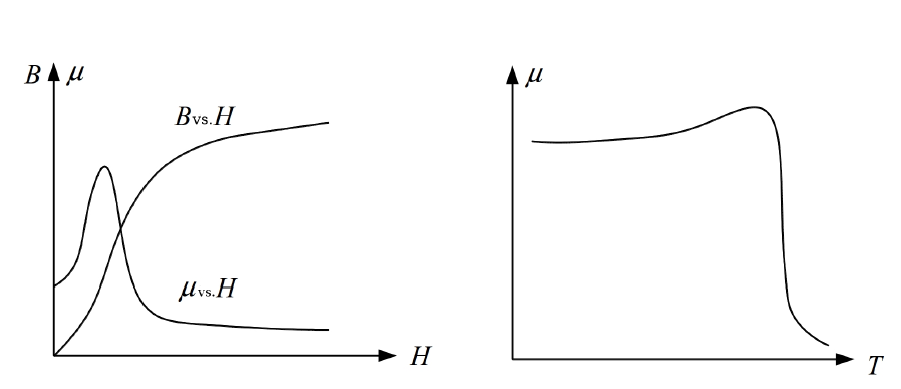
\includegraphics[scale=0.5]{P1.jpg}
\caption{(left) The magnetization curve $B(H)$ for a ferromagnetic material and the
curve $\mu(H)$. (right) A generic graph of the $\mu(T)$ curve for a ferromagnetic material.}
\end{figure}
The magnitudes of the magnetic field and the auxiliary magnetic field are related
linearly in non-ferromagnetic isotropic materials, that is in such materials $B = \mu H$. How-
ever, for ferromagnetic materials the relationship is non-linear. In ferromagnetic materials
there is a spontaneous magnetization (magnetic dipole moments are spontaneously oriented parallel to each other) that increases with the decreasing temperature. Figure 1
(left) shows a typical magnetization curve $B = B(H)$ with some features common to all
ferromagnetic materials. Namely, when $H$ increases, $B$ increases slowly at the beginning
and $\mu$ is small; then $B$ and $\mu$ both rapidly increase as $H$ increases; finally, $B$ reaches a saturation level and $\mu$ rapidly decreases after reaching a maximum value. Figure 1 indicates that the magnetic permeability $\mu$ is a function of both the auxiliary magnetic field $H$ (Figure 1, left) and the temperature $T$ (Figure 1, right).
\par If the temperature is increased above a certain value, a ferromagnet will turn into a paramagnet, that is a material with randomly oriented magnetic dipole moments. This critical value of the temperature is called the $Curie$ $temperature$, and on the graph $\mu$ vs.
$T$ it is the temperature corresponding to the point where the slope of the tangent line is
maximum.
\subsection{Magnetic Hysteresis}
In addition to high magnetic permeability, ferromagnets have another important property, which is the magnetic hysteresis. When a ferromagnet is being magnetized, the
magnetic field $B$ depends not only on the current value of the auxiliary magnetic field
H, but also on the previous state of the material, as shown in Figure 2. The curve $OA$,
where the magnetic field $B$ grows as the auxiliary magnetic field $H$ increases, describes
the process of magnetizing of an (initially demagnetized) ferromagnet. This curve is called
the $magnetization$ $curve$.
\par When the auxiliary magnetic field is increased to a certain value $H_S$, the magnetic field $B$ hardly increases and reaches a saturation state. If then the auxiliary magnetic field is being decreased, the magnetic field $B$ is not decreasing along the original path, but rather choosing another path $AC'A'$. Furthermore, when $H$ increases from the value $-HS$, $B$
will reach $A$ along the curve $A'CA$, and finally form a closed curve. When $H$ = 0, we
have $|B|=B_r$, where $B_r$ is called the $remnant$ $magnetic$ $field$ (yielding the corresponding remnant magnetization). In order to make $B=0$, an auxiliary magnetic field has to be applied in the reverse direction. When the auxiliary magnetic field reaches the value
$H=-H_C$, where $H_C$ is called the coercive field strength, the material is demagnetized
and the magnetic field $B$, and hence the magnetization, is zero. Different ferromagnetic materials have different magnetic hysteresis loops with different values of the coercive auxiliary field strengths. Ferromagnetic materials with a large value of the coercive auxiliary  field are called $hard$ magnetic materials, whereas those with a small one classified as $soft$ magnetic materials.
\begin{figure}[H]
\centering
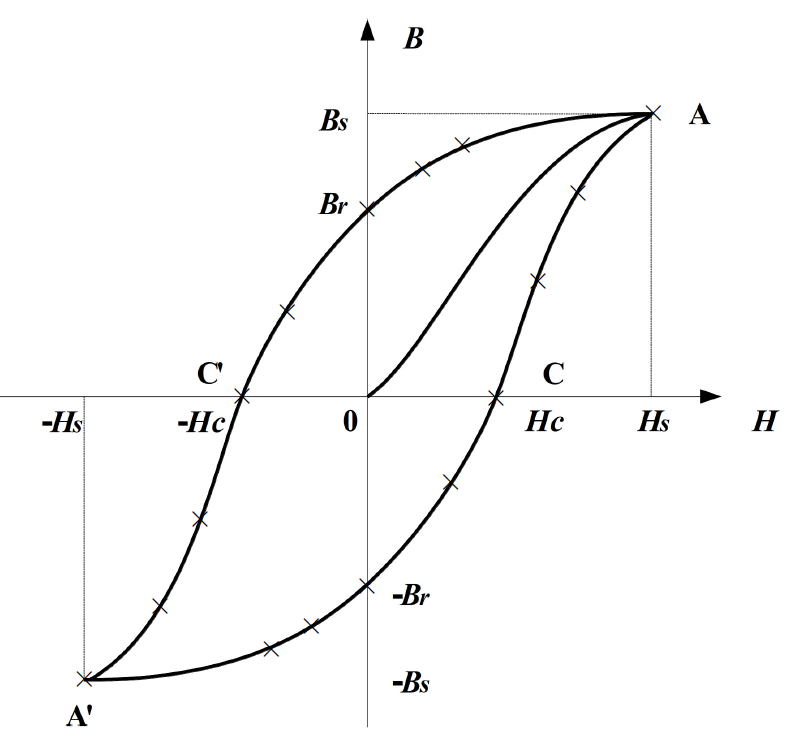
\includegraphics[scale=0.3]{P2.jpg}
\caption{The magnetization curve and the magnetic hysteresis loop of a ferromagnetic
material. The crosses indicate the points to be recorded to describe the loop.}
\end{figure}
\subsection{Visualization on the Oscilloscope}
\begin{figure}[H]
\centering
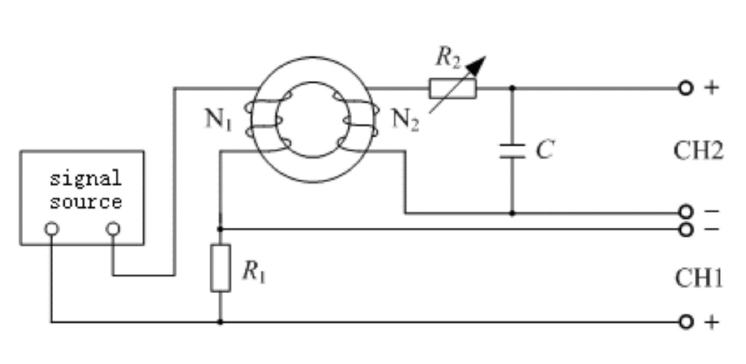
\includegraphics[scale=0.5]{P3.jpg}
\caption{The electric circuit for visualization of the magnetization curve and the magnetic
hysteresis loop on the oscilloscope.$R_1=10\Omega$ and $R_2$ is a variable resistor with maximum resistance of 2.2 k$\Omega$.}
\end{figure}
Figure 3 presents a diagram of a circuit that is used to visualize the magnetization
curve and the magnetic hysteresis loop on the oscilloscope. In this exercise they are
studied for a ferromagnet sample that has an average magnetic path of $L$ and the number
of the turns in the coil is $N_1$. If the electric current through the coil is $i_1$, then according to Amp$\grave{e}$re's law$$HL=N_1i_1$$In this case the input voltage for the deflection plate of the $x$ axis channel of the oscilloscope is 
$$U_{R_1}=R_1i_1=\frac{R_1L}{N_1}H$$
where $R_1,L,$ and $N_1$ are constant. Hence, the input voltage for the $x$ axis channel is
proportional to the auxiliary magnetic field $H$.
\par If the cross-sectional area of the sample is $S$, then according to the law of electromagnetic induction, the induced electromotive force in a secondary coil with the number of turns $N_2$, is 
\begin{equation}
\varepsilon_2=-N_2S\frac{\mathrm{d}B}{\mathrm{d}t}
\end{equation}
Assuming that the number of turns $N_2$ in the secondary coil is small, the electromotive
force due to self-induction can be ignored. Moreover, if the values of the resistance $R_2$
and the capacitance $C$ are chosen so that $R_2\gg1/\varepsilon C$, then
\begin{equation}
\varepsilon_2=R_2i_2
\end{equation}
Substituting $i_2=\frac{\mathrm{d}q}{\mathrm{d}t}=C\frac{\mathrm{d}U_c}{\mathrm{d}t}$ into Eq. (2) and combining with Eq.(1) one obtains $$U_C=-\frac{N_2SB}{R_2C}$$which shows that the input voltage $U_C$ for the $y$ axis channel is proportional to the magnetic field $B$.
\subsection{Measurement of the Curie Temperature with an Alternating Current Bridge}
An alternating-current (AC) bridge can be used to measure the Curie temperature of
a ferromagnetic material. Although there are many variations of AC bridges, such as the
Maxwell bridge, the Owen bridge, etc, the basic working principle can be illustrated with
a four-side impedance bridge as shown in Figure 4.
\begin{figure}[H]
\centering
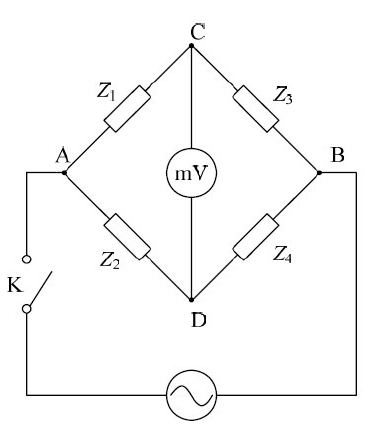
\includegraphics[scale=0.5]{P4.jpg}
\caption{Four-side impedance bridge.}
\end{figure}
The four sides of the bridge are combinations of resistive, capacitive, and inductive
elements combined in series or in parallel. The idea is to adjust the parameters of the
bridge in order to eliminate a potential difference between the points $C$ and $D$. When
the bridge reaches this equilibrium state, one should have
$$\frac{Z_1}{Z_2}=\frac{Z_3}{Z_4}$$
To make this equality hold, the moduli and the phases of both sides should be equal,$i.e$.
$$\frac{|Z_1|}{|Z_2|}=\frac{|Z_3|}{|Z_4|},\varphi_1+\varphi_4=\varphi_2+\varphi_3$$
respectively. Then the bridge is balanced, $i.e$. the potential difference between the points
$C$ and $D$ is equal to zero.
\par Figure 5 shows a $RL$ $AC$ bridge used in this experiment. The input current source is
supplied by a signal generator, allowing to chose a suitable (high) output frequency. The
elements $Z_1$ and $Z_2$ are resistors, whereas $Z_3$ and $Z_4$ are inductors with a finite resistance $r_1$ and $r_2$, respectively. The impedances of these four elements are
$$Z_1=R_1,Z_2=R_2,Z_3=r_1+j\omega L_1,Z_4=r_2+j\omega L_2$$
with $j$ being the imaginary unit $(j^2=-1)$ and $\omega——$ the angular frequency of the signal
provided by the voltage source. When the bridge is in balance $$r_2=\frac{R_2}{R_1}r_1,L_2=\frac{R_2}{R_1}L_1$$
\begin{figure}[H]
\centering
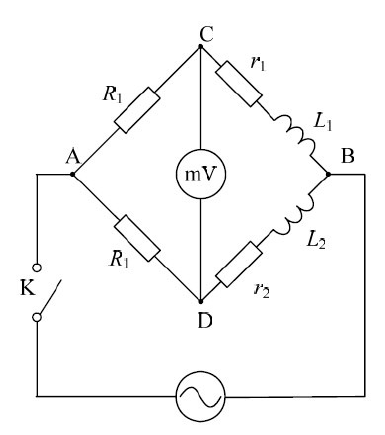
\includegraphics[scale=0.5]{P5.jpg}
\caption{AC bridge}
\end{figure}
First, the AC bridge with the ferromagnetic sample removed needs to be balanced by
adjusting parameters of the circuit components. After the sample is placed in the apparatus, the balance will be broken because of the resulting change in the inductance. Then,
when the temperature is increased to the critical value, the ferromagnet undergoes a transition to the paramagnetic state, the potential difference between $C$ and $D$ will suddenly
becomes nearly zero again and at this very point the balance is recovered. This particular
transition point allows one to estimate the Curie temperature, $i.e$. the temperature of
the ferromagnetic-paramagnetic phase transition, by observing the voltage-temperature
curve.
\par In this exercise, the right half $(r1, L1, r2$ and $L2)$ of the AC bridge, along with the
temperature probe, is placed in a glass vacuum-tube heating pipe. Heating is provided
by a voltage/current source and Series voltage sources mode should be chosen. The tube
should be heated starting from the room temperature to about $60^oC$ by using moderate
values of the voltage (about 7 V each, obtained from the test). It is important to wait
for the system to reach a thermal balance (waiting time is about 5 minutes), and then
gradually increase the input voltage so that the temperature rises slowly enough (that is
the value of $U_{CD}$ does not change too fast). If the heating process is too fast, the temperature probe and the sample will have different temperatures, resulting in an inaccurate
measurement. This is especially important when the temperature gets close to the Curie
temperature; the measurement will be inaccurate if the voltage $U_{CD}$ is not changing slowly
enough.
\section{Apparatus}
The apparatus for this exercise consists of the following main elements: a signal generator, an oscilloscope, a digital multimeter, a platinum resistance thermometer, a glass
vacuum-tube heating pipe, a voltage/current source, a wiring block, a capacitor, two 200$\Omega$ resistors, a 10$\Omega$ resistor, a 2.2 k$\Omega$ variable resistor, and a 1k$\Omega$ resistor (the actual values of the resistance should be measured during the session). Ferromagnetic samples will be provided by the instructor.
\par The parameters of other elements are: $L=3.61\cdot10^{-2}$m, $S=1.25\cdot10^{-5}$m$^2$ and $N_1=N_2=100.$ The capacity is indicated on the capacitor.
\section{Procedure}
\subsection{Magnetic Hysteresis Loop Measurement}
\begin{enumerate}
\item Assemble the circuit according to Figure 3 with the signal source disconnected.
\item Turn on the signal source and adjust the frequency to 1 kHz or above. Keep in
mind that you must not short the signal source, or set the frequency below 1 kHz
(otherwise the equipment will be damaged).
\item Connect the signal source to the circuit and observe the $U_{R_1}$ vs. $U_C$ loop under
different conditions:
\begin{enumerate}[(1)]
\item with different signal frequencies (1$\sim$2 kHz) and amplitudes (1$\sim$5 V),
\item with different values of the resistance $R_2$.
\end{enumerate}
\item Obtain the saturated hysteresis loop for a certain frequency (1$\sim$2 kHz) and
suitable value of the resistance $R_2$ (about 1 k$\Omega$); shift the picture of the loop to the center of the oscilloscope screen, adjust its size and show the visualization to the
instructor.
\item Trace the whole loop with no less than 16 points (see Figure 2 for the location of
the points).
\item Turn off the signal source, disconnect the circuit and measure the resistances.
\item After class, plot the magnetic hysteresis loop ($H——B$ loop), and find $\pm B_r,\pm H_c, \pm B_s,\pm H_s.$
\end{enumerate}
\subsection{Measurement of the Curie Temperature with an AC Bridge}
\begin{enumerate}
\item Properly set the AC measurement range on the multimeter and assemble the circuit
according to Figure 5.
\item A small piece of the ferromagnetic sample will be provided by the instructor. Study the circuit without heating up the sample. Note the differences before and after
placing the ferromagnetic sample in the coil.
\item Put the right half of the AC bridge (two coils, one of the coils should contain the
ferromagnetic sample) into the heating pipe. Set the voltage/current source in the
Series mode to heat up the tube. Adjust the voltages to 7 V each and wait for
about 5 minutes for the thermal balance at about 60$^o$C (approximate value; may
differ due to the changes in the room temperature and different resistances of the
heaters). Record T vs. $U_{CD}$ with intervals of about $5^o$C during this step if $U_{CD}$ is not changing too fast.
\item After the first thermal balance is reached, slightly increase the voltage of the sources
by about 0:5 V each. Above 60$^o$C, record T vs. $U_{CD}$ with intervals of about 0.1$^o$C
and make sure that $U_{CD}$ is not changing too fast. Continue recording until the
thermal balance is reached again.
\item Repeat Step 4 several times until the change of $U_{CD}$ with $T$ is sufficiently small
(above ca. 80$^o$C).
\item Disconnect the circuit, wait for the tube to cool down and remove the coils from
the pipe; return the ferromagnetic sample to the instructor.
\item After class, use a computer to plot the $U_{CD}$ vs. T curve and the $\bigtriangleup U_{CD}=\bigtriangleup T$ vs. $T$ curve to identify the Curie temperature (as the temperature for which the ratio$\bigtriangleup U_{CD}=\bigtriangleup T$ is minimum).
\end{enumerate}
\section{Results and Calculation}
\subsection{Parameters of Circuit Components}
\begin{table}[H]
\centering
\begin{tabular}{|c|c|}
\hline
$N_1$ &100  \\ \hline
$N_2$ &100  \\ \hline
$R_1$ &$10.78\pm 0.01[\Omega]$  \\ \hline
$R_2$ &$219.49\pm 0.01[\Omega]$  \\ \hline
$L$ &$3.61\times10^{-2}\pm0.01\times10^{-2}[m]$  \\ \hline
$S$&$1.25\times10^{-5}\pm0.01\times10^{-5}[m^2]$  \\ \hline
$C$&$4.345\pm0.001[\mu F]$  \\ \hline
\end{tabular}
\caption{Parameters of circuit components}
\end{table}
\subsection{Oscilloscope-measured values of $U_{R_1}$ and $U_C$}
\begin{table}[H]
\centering
\begin{tabular}{|c|c|}
\hline
$U_{R_1}(\pm 0.001[V])$ &$U_C(\pm 0.001[V])$  \\ \hline
-0.350 &-0.650  \\ \hline
-0.250 &0.000  \\ \hline
-0.000 &0.600  \\ \hline
0.320 &0.800  \\ \hline
0.190 &0.000  \\ \hline
0.000 &-0.410  \\ \hline
-0.290 &-0.500  \\ \hline
-0.100 &0.500  \\ \hline
0.240 &0.500  \\ \hline
-0.130 &-0.500  \\ \hline
0.170 &-0.120  \\ \hline
-0.270 &-0.120  \\ \hline
-0.210 &0.290  \\ \hline
0.220 &0.290  \\ \hline
-0.020 &0.580  \\ \hline
0.240 &0.580  \\ \hline
\end{tabular}
\caption{Oscilloscope-measured values of $U_{R_1}$ and $U_C$ in the circuit}
\end{table}
\subsection{Calculation of $B$ and $H$}
$$H_1=\frac{U_{R_1}N_1}{R_1 L}=\frac{-0.350\times100}{10.78\times3.61\times10^{-2}}=-89.9[A/m]$$
$$B_1=-\frac{U_c R_2 C}{N_2 S}=-\frac{-0.650\times219.49\times4.345}{100\times 1.25\times10^{-5}}=0.496[A/m]$$
\begin{table}[H]
\centering
\begin{tabular}{|c|c|}
\hline
$H[A/m]$ &$B[A/m]$  \\ \hline
-89.9 &0.496  \\ \hline
-64.2 &0.000  \\ \hline
0.00 &-0.458  \\ \hline
82.2 &-0.610  \\ \hline
48.8 &0.000  \\ \hline
0.00 &0.313  \\ \hline
-74.5 &0.381  \\ \hline
-25.7 &-0.381 \\ \hline
61.7 &-0.381  \\ \hline
-33.4 &0.381  \\ \hline
43.7 &0.0916 \\ \hline
-69.4 &0.0916  \\ \hline
-54.0 &-0.221  \\ \hline
56.5 &-0.221  \\ \hline
-5.14 &0.443  \\ \hline
61.7 &0.443 \\ \hline
\end{tabular}
\caption{Oscilloscope-measured values of $U_{R_1}$ and $U_C$ in the circuit}
\end{table}
\section{Uncertainty Analysis}
\subsection{Uncertainty of $H$}
$$u_H=\sqrt{(\frac{\partial B}{\partial U_u}u_u)^2+(\frac{\partial H}{\partial R_1}u_R)^2+(\frac{\partial H}{\partial L}u_L)^2}$$
$$\sqrt{(\frac{100}{10.78\cdot3.61}\cdot10^{-1})^2+(\frac{0.35\cdot100}{(10.78)^2\cdot3.61})^2+(\frac{0.35\cdot100}{10.78\cdot(3.61)^2})^2}$$
$$u_H=9.6\cdot10^{-2},u_r=\frac{u_H}{H}\cdot100\%=0.11\%$$
$$H_1=-89.9\pm9.6\cdot10^{-2}[A/m]$$
\begin{table}[H]
\centering
\begin{tabular}{|c|c|c|}
\hline
$H[A/m]$ & $u_H[A/m]$ &$u_r\%$  \\ \hline
-89.9&$9.6\cdot10^{-2}$  &$0.11\%$  \\ \hline
-64.2 &$5.3\cdot10^{-2}$  &$0.08\%$  \\ \hline
0.00 &$6.6\cdot10^{-2}$  &$0.00\%$    \\ \hline
82.2 &$9.3\cdot10^{-2}$  &$0.11\%$    \\ \hline
48.8 &$8.1\cdot10^{-2}$  &$0.17\%$  \\ \hline
0.00 &$6.6\cdot10^{-2}$  &$0.00\%$    \\ \hline
-74.5&$5.2\cdot10^{-2}$  &$0.07\%$    \\ \hline
-25.7&$6.0\cdot10^{-2}$  &$0.23\%$    \\ \hline
61.7&$8.5\cdot10^{-2}$  &$0.14\%$    \\ \hline
-33.4&$7.6\cdot10^{-2}$  &$0.23\%$    \\ \hline
43.7&$7.9\cdot10^{-2}$  &$0.18\%$    \\ \hline
-69.4&$8.8\cdot10^{-2}$  &$0.13\%$    \\ \hline
-54.0&$8.2\cdot10^{-2}$  &$0.15\%$    \\ \hline
56.5&$8.3\cdot10^{-2}$  &$0.15\%$    \\ \hline
-5.14 &$6.7\cdot10^{-2}$  &$1.30\%$    \\ \hline
61.7 &$8.5\cdot10^{-2}$  &$0.14\%$    \\ \hline
\end{tabular}
\caption{Uncertainty of $H$}
\end{table}
\subsection{Uncertainty of $B$}
$$u_B=\sqrt{(\frac{\partial B}{\partial U_c}u_u)^2+(\frac{\partial B}{\partial R_2}u_R)^2+(\frac{\partial B}{\partial C}u_c)^2+(\frac{\partial B}{\partial s}u_s)^2}$$
$$\sqrt{(\frac{219.49\cdot4.345\cdot10^{-6}}{1.25})^2+(\frac{0.65\cdot4.345\cdot10^{-5}}{1.25})^2+(\frac{0.65\cdot219.49}{1.25}\cdot10^{-6})^2+(\frac{0.65\cdot219.49\cdot4.345}{(1.25)^2}\cdot10^{-5})^2}$$
$$u_B=4.04\cdot10^{-3},u_r=\frac{u_B}{B}\cdot100\%=0.81\%$$
$$B_1=0.496\pm4.04\cdot10^{-3}[A/m]$$
\begin{table}[H]
\centering
\begin{tabular}{|c|c|c|}
\hline
$B[A/m]$ & $u_B[A/m]$ &$u_r\%$  \\ \hline
0.496 &$4.0\cdot10^{-3}$  &$0.81\%$  \\ \hline
0.000 &$0.8\cdot10^{-3}$  &$0.00\%$  \\ \hline
-0.458 &$3.7\cdot10^{-3}$  &$0.81\%$    \\ \hline
-0.610 &$4.9\cdot10^{-3}$  &$0.80\%$    \\ \hline
0.000 &$0.8\cdot10^{-3}$  &$0.00\%$  \\ \hline
0.313 &$2.6\cdot10^{-3}$  &$0.83\%$    \\ \hline
0.381&$2.4\cdot10^{-3}$  &$0.63\%$    \\ \hline
-0.381&$2.4\cdot10^{-3}$  &$0.63\%$    \\ \hline
-0.381&$2.4\cdot10^{-3}$  &$0.63\%$    \\ \hline
0.381&$2.4\cdot10^{-3}$  &$0.63\%$    \\ \hline
0.0916&$1.1\cdot10^{-3}$  &$1.2\%$    \\ \hline
0.0916&$1.1\cdot10^{-3}$  &$1.2\%$    \\ \hline
-0.221&$1.9\cdot10^{-3}$  &$0.86\%$    \\ \hline
-0.221&$1.9\cdot10^{-3}$  &$0.86\%$    \\ \hline
0.443 &$3.6\cdot10^{-3}$  &$0.81\%$    \\ \hline
0.443 &$3.6\cdot10^{-3}$  &$0.81\%$    \\ \hline
\end{tabular}
\caption{Uncertainty of $B$}
\end{table}
\subsection{Plot of $B$ vs. $H$}
\begin{figure}[H]
\centering
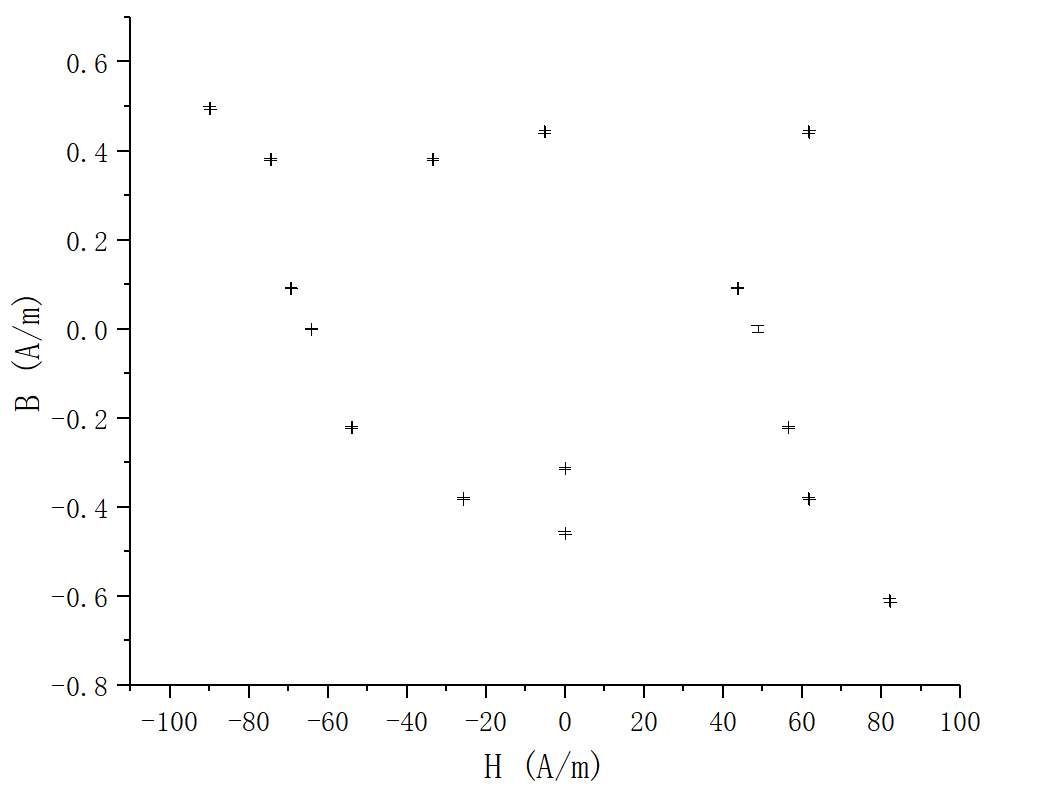
\includegraphics[scale=0.4]{P6.jpg}
\caption{Plot of $B$ vs. $H$}
\end{figure}
\begin{table}[H]
\centering
\begin{tabular}{|c|c|c|c|}
\hline
quantity &  $[A/m]$      & $u[A/m]$   & $u_r [\%]$ \\ \hline
$B_s$     & 0.496  & $4.0\cdot 10^{-3}$ & $0.81\%$ \\ \hline
$-B_s$    & -0.610 &$4.9\cdot 10^{-3}$ & $0.80\%$ \\ \hline
$H_s$     & -89.9  & $9.6\cdot 10^{-2}$ & $0.11\%$ \\ \hline
$-H_s$    & 82.2   & $9.3\cdot 10^{-2}$ & $0.11\%$ \\ \hline
$H_c$     & -64.2  & $5.3\cdot 10^{-2}$ & $0.08\%$ \\ \hline
$-H_c$    & 48.8   & $8.1\cdot 10^{-2}$ & $0.17\%$\\ \hline
$B_r$     & 0.313  & $3.9\cdot 10^{-3}$ & $0.81\%$\\ \hline
$-B_r$    & -0.458 & $2.6\cdot 10^{-3}$ & $0.83\%$\\ \hline
\end{tabular}
\caption{Data for $\pm B_s,\pm H_s,\pm H_c,\pm B_r$}
\end{table}
\section{Conclusion}
\par Through this lab work, I have a rough idea about basic characteristic of magnetic materials. I become familiar with paramagnetic and ferromagnetic materials. I know the magnetic hysteresis loop, a distinct characteristic of ferromagnetic materials.
\par In this experiment, I built a circuit to measure $B$ and $H$ indirectly by measure the voltage of the capacitor and resistor, then make a plot of $B$ and $H$.
 My plot is opposite to the figure in lab manual, I think it's because $U_C=-\frac{N_2 SB}{R_2C}$, which makes the figure is opposite to the picture on the oscilloscope.
\par In the second part of the experiment, we're asked to measure the Curie Temperature by building the four-side impedance bridge. But, we didn't do it due to the time limit but I still learn a lot of thing about the Curie Temperature of ferromagnetic materials.
\subsection{Error Analysis}
The relative uncertainty is not very big, but it becomes bigger as $B$ and $H$ becomes smaller. In addition, my plot is not symmetric enough, I think the error is caused by the oscilloscope. When I use the oscilloscope, I put the center of the graph at the center of the monitor but after I start measuring, it moved away, so the whole graph was changed. 
\subsection{Improvement}
\begin{enumerate}
\item I should measure more value of $B$ and $H$ next time because I measured too much points with same $B$ and $H$, which may cause more error.
\item When I use the Oscilloscope next time, I should pay more attention to the position of the figure to make sure I get the correct picture.
\end{enumerate}
\section{Data Sheet}
Data sheet is attach to the report
\section{Reference}
\par Young, H.D., Freedman R.A. University Physics. Chapter 28,31.
\par Krzyzosiak,M. Lab Manual of Exercise 1.
\par Qin Tian, Zeng Ming, Zhao Xijian, Krzyzosiak,M. Handbook-Uncertainty Analysis.
\end{document}